\section{Auswertung}
\label{sec:Auswertung}

In Abbildung \ref{fig:oszi1_2} ist eine typische Aufnahme eines Sweep-Durchgangs bei einer Frequenz von $\SI{100}{\kilo \hertz}$ zu sehen. Die Ordinate ist proportional zur Transparenz des Rubidiumdampfes für das eingestrahlte rechtszirkular polarisierte Licht und die Abszisse ist proportional zum Magnetfeld, welches durch die beiden horizontalen Spulen erzeugt wird. Die zu beobachtenden Minima in der Transparenz entsprechen von links nach rechts dem Nulldurchgang des Magnetfelds, der Resonanzstelle des ersten Rubidium-Isotops und der Resonanzstelle des zweiten Rubidium-Isotops. Beim verschwindenden Magnetfeld ist die Transparenz des Dampfes am geringsten, da dann keine Zeeman-Aufspaltung der Energieniveaus auftritt und somit kein optisches Pumpen möglich ist.

\begin{figure}[h]
\centering
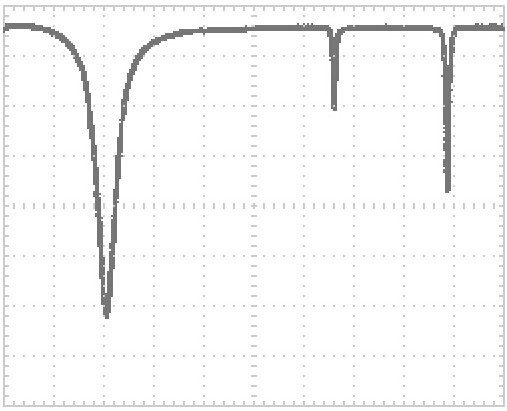
\includegraphics[width=0.7\linewidth]{img/oszi1_2}
\caption{Typische Aufnahme auf dem Oszilloskop bei einer Frequenz von $\SI{100}{\kilo \hertz}$. Aufgetragen ist die Transparenz des Rubidiumdampfes in Abhängigkeit vom angelegten Magnetfeld. Die drei Minima entsprechen von links nach rechts einem verschwindenden Magnetfeld und den Resonanzstellen der beiden Rubidium-Isotope beim optischen Pumpen.}
\label{fig:oszi1_2}
\end{figure}

Die Magnetfelder, bei denen zu den eingestellten Frequenzen Minima der Transparenz des Dampfes auftreten, sind in Abbildung \eqref{fig:plot1} in Abhängigkeit von den jeweiligen Frequenzen dargestellt. Die dazu aufgenommenen Messdaten lassen sich den Tabellen \ref{tab:tab1} und \ref{tab:tab2} entnehmen, wobei die Ungenauigkeiten in den Frequenzen und Stromstärken auf Grundlage des Spiels an den Drehreglern der verwendeten Apparaturen abgeschätzt wurden. Die Magnetfelder wurden nach der bekannten Beziehung 

\begin{equation}
	B = \mu_0 \frac{8}{\sqrt{125}} \frac{N \cdot I}{R}
	\label{helm}
\end{equation}

für das Magnetfeld in einer Helmholtzspule in Abhängigkeit von deren Radius $R$ und Strom $I$ zur Magnetfelderzeugung  ermittelt und die zugehörigen Fehler mittels Gauß'scher Fehlerfortpflanzung und der Programmbibliothek SciPy \cite{SciPy} bestimmt. Über eine lineare Regressionsgerade der Form $B(f) = a \cdot f + b$ werden die \eqref{ABC} überprüft und die entsprechenden Parameter bestimmt:

\begin{figure}
	\centering
	\caption{Plot der Messdaten der Resonanzstellen und linearen Regressionsgeraden. Die Zuordnung der beiden Isotope mit den beiden Resonanzstellen wird im Folgenden beschrieben.}
	\includegraphics[width=0.9\linewidth]{img/plot1}
	\label{fig:plot1}
\end{figure}

\input{tab/tab1}

\input{tab/tab2}

\begin{eqnarray}
	a_1 =& \SI{1.42 \pm 0.01 e-10}{\tesla \hertz^{-1}} &a_2 =  \SI{2.11 \pm 0.01 e-10}{\tesla \hertz^{-1}}\\
	b_1 =& \SI{4.55 \pm 0.09 e-5}{\tesla}  &b_2 = \SI{4.59 \pm 0.08 e-5}{\tesla} 
\end{eqnarray}

Da der Versuchsaufbau in der Horizontalen parallel zu den magnetischen Feldlinien des Erdmagnetfelds ausgerichtet wurde, wird die Ordinatenachse effektiv um den horizontalen Anteil des Erdmagnetfelds verschoben. Mittelung über $b_1$ und $b_2$ ergibt:

\begin{equation}
	B_\text{Erde,\,hor} = \SI{45.7\pm 0.6}{\micro \tesla}.
\end{equation}

Die Steigung der Regressionsgeraden ist nach \eqref{ABC} antiproportional zum gesuchten Landé-Faktor $g_F$ der beiden Isotope. Mit $g_F = \frac{h}{\mu_B} \frac{1}{a}$ ergibt sich für die beiden Isotope:

\begin{eqnarray}
	g_{F,1} = \SI{0.505 \pm 0.005},\\
	g_{F,2} = \SI{0.337 \pm 0.002}.
\end{eqnarray}

Nun lässt sich der Kernspin der beiden Isotope durch \eqref{eqn:g_F} bestimmen, wobei der Landé-Faktor $g_J$ des Elektrons benötigt wird. Dieser kann nach \eqref{GHI} durch Einsetzen der Quantenzahlen $S = \frac{1}{2}, L = 0$ und $J = \frac{1}{2}$ berechnet werden. Wird $F = I + J$ verwendet\footnote{$F$ nimmt diesen maximalen Wert an, da nur für das Niveau mit dem höchstmöglichen $m_F$ kein Übergang durch das optische Pumpen möglich ist.}, ergibt sich die Relation

\begin{equation}
	I = \frac{1}{2} \left(\frac{g_J}{g_F} - 1\right)
\end{equation}

für den Kernspin der beiden Isotope. Einsetzen der Messwerte ergibt

\begin{eqnarray}
	I_1 = \SI{1.48 \pm 0.02},\\
	I_2 = \SI{2.47 \pm 0.02}.
\end{eqnarray}

Ein Vergleich mit den Literatur-Werten $I_{{}^{85}\text{Rb,\,lit}} = 2.50$ und $I_{{}^{87}\text{Rb,\,lit}} = 1.50$ \cite{Rb} für den Kernspin der Rubidium Isotope lässt eine Identifizierung der Isotope zu: Die mit dem Index $1$ gekennzeichnete Resonanz wird durch das Vorhandensein des Isotops ${}^{87}\text{Rb}$ im untersuchten Dampf verursacht und die mit $2$ gekennzeichnete durch das Vorhandensein des Isotops ${}^{84}\text{Rb}$.

Die Anteile der Isotope $P_{\text{Rb}85}$ und $P_{\text{Rb}87}$ können näherungsweise aus dem Verhältnis der Tiefen der Dips in Abbildung \ref{fig:oszi2_3} bestimmt werden. Annahme soll dabei sein, dass der untersuchte Dampf ausschließlich aus den beiden Isotopen besteht: $P_{\text{Rb}85} + P_{\text{Rb}87} = 1$. Auszählen der Pixel in der Bildbearbeitungssoftware GIMP \cite{Gimp} mit einer abgeschätzten Ungenauigkeit von zwei Pixeln aufgrund der unscharfen Ränder der Dips ergibt:


\begin{figure}
	\centering
	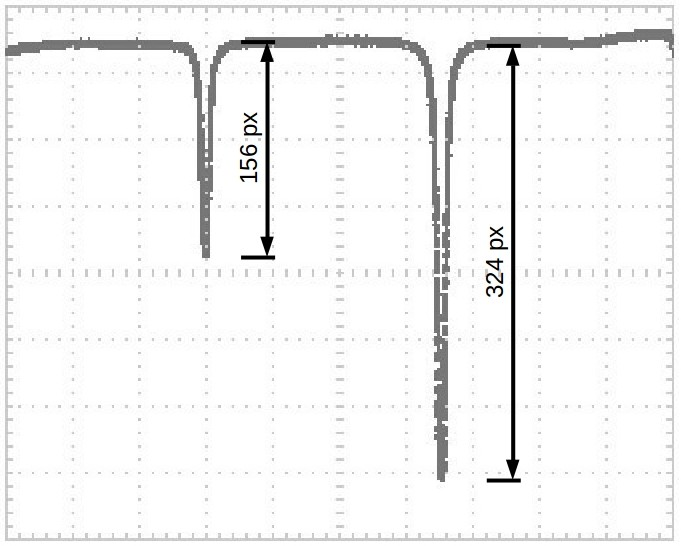
\includegraphics[width=0.7\linewidth]{img/oszi2_3}
	\caption{Screenshot des Oszilloskops mit Fokus auf die beiden Resonanzsstellen. Die gemessenen Tiefen der Dips wurden mit der Bildbearbeitungssoftware GIMP eingefügt.}
	\label{fig:oszi2_3}
\end{figure}

\begin{eqnarray}
	N_{\text{Rb}87} = (156 \pm 2)\, \text{px},\\
	N_{\text{Rb}85} = (324 \pm 2)\, \text{px}
\end{eqnarray}

Es ergibt sich das Verhältnis $R = \frac{P_{\text{Rb}87}}{P_{\text{Rb}85}} = \frac{N_{\text{Rb}87}}{N_{\text{Rb}85}}$, woraus

\begin{eqnarray}
	P_{\text{Rb}87} = \frac{R}{1 + R} = (32.5 \pm 0.3) \%, \\
	P_{\text{Rb}85} = 1 - P_{\text{Rb}87} = (67.5 \pm 0.3) \%
\end{eqnarray}

folgt.

Der quadratische Zeeman-Effekt ist in diesem Versuch nicht von Relevanz. Dies lässt sich 
durch die folgende kurze Rechnung nach Gleichung \eqref{quad} demonstrieren: Da der quadratische 
Zeeman-Effekt erst für große Magnetfelder $B$ relevant wird, wird für die Abschätzung das 
größte in diesem Versuch berechnete Magnetfeld von $B = \SI{257}{\micro \tesla}$ verwendet. Für die 
Landé-Faktoren werden die ermittelten Werte verwendet. Für die Quantenzahl $m_F$ werden auch
 jeweils die größtmöglichen gewählt: $m_{F, \, \text{Rb}85} = 3$ und $m_{F, \, \text{Rb}87} = 2$.
  Die Hyperfeinaufspaltung ist mit $\Delta E_{\text{Hy}, \, \text{Rb}85} = {2.01 \cdot 10^{-24}}\, \text{J}$ und
   $\Delta E_{\text{Hy}, \, \text{Rb}87} = {4.53 \cdot 10^{-24}}\, \text{J}$ gegeben \cite{V21}.
   Demnach gilt: 
    $U_{\text{HF}, \, \text{Rb}85}^\text{lin} = {(8.04 \pm 0.05) \cdot 10^{-28}}\, \text{J}$ und 
    $U_{\text{HF}, \, \text{Rb}85}^\text{quad} = {(-7.14 \pm 0.09) \cdot 10^{-31}}\, \text{J}$ sowie
     $U_{\text{HF}, \, \text{Rb}87}^\text{lin} = {(1.20 \pm 0.01) \cdot 10^{-27}}\, \text{J}$ und
     $U_{\text{HF}, \, \text{Rb}87}^\text{quad} = {(-3.60 \pm 0.08) \cdot 10^{-31}}\, \text{J}$. 
     Die linearen Terme liegen also betragsmäßig mindestens zwei Größenordnungen über den Beiträgen hoher Magnetfelder. 